\section{Syntax analysis and parsing}

Consider the following grammar $G$, represented as a machine net over the two-letter terminal alphabet $\Sigma = \{ a, b \}$ and the two-letter non-terminal alphabet 
$V = \{ S, A \}$ (axiom $S$).
\begin{figure}[H]
    \centering
    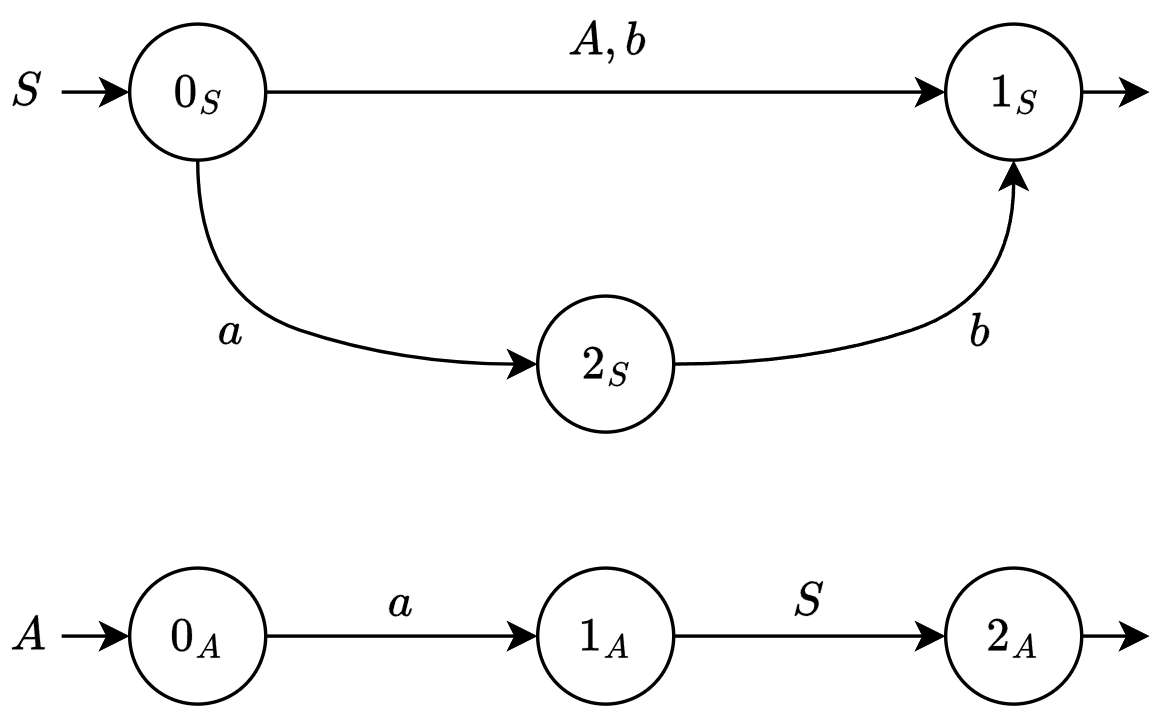
\includegraphics[width=0.5\linewidth]{images/parsing.png}
\end{figure} 
Answer the following questions:
\begin{enumerate}
    \item Draw the syntax tree (or trees if there are two or more) of the valid string $a a b$.
    \item Draw the complete pilot of grammar $G$, say if grammar $G$ is of type ELR (1), and shortly justify your answer. 
        If the grammar is not ELR(1) then highlight all the conflicts in the pilot.
    \item Write all the guide sets on the arcs of the machine net (shift and call arcs, and final arrows), say if grammar G is of type ELL(1), based on the guide sets, and shortly justify your answer. 
        If you wish, you can use the figure above to add the call arcs and annotate the guide sets.
    \item Analyze the valid string $a a b$ using the Earley method; show the item/all the items that gives/give evidence of string acceptance.
\end{enumerate}

\paragraph*{Solution}
\begin{enumerate}
    \item The string $aab$ exhibits ambiguity, leading to two distinct syntax trees:
        \begin{figure}[H]
            \centering
            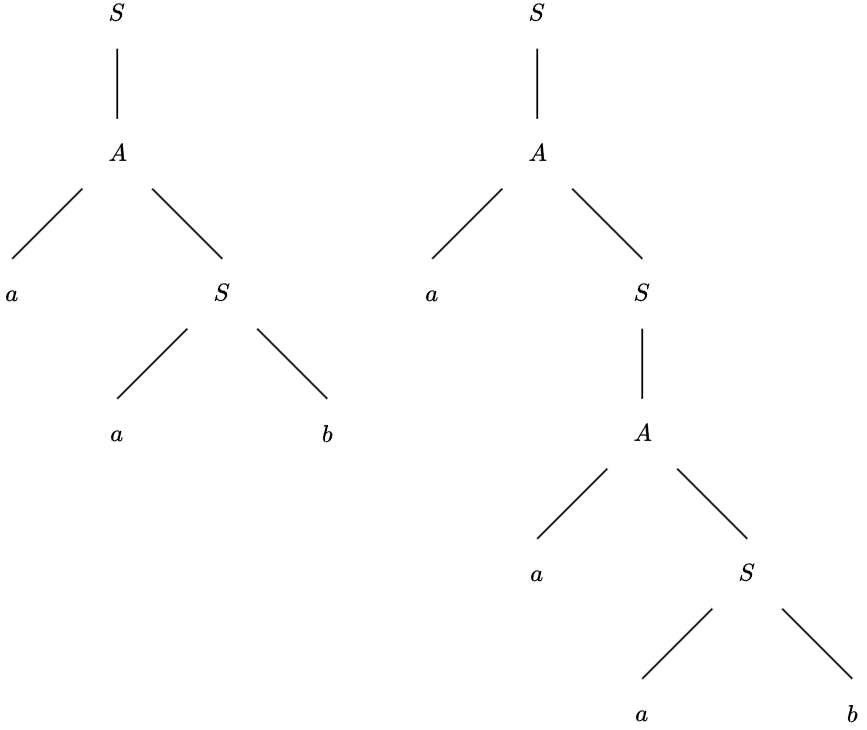
\includegraphics[width=0.75\linewidth]{images/syntax.png}
        \end{figure} 
    \item The pilot for the given grammar is as follows:
        \begin{figure}[H]
            \centering
            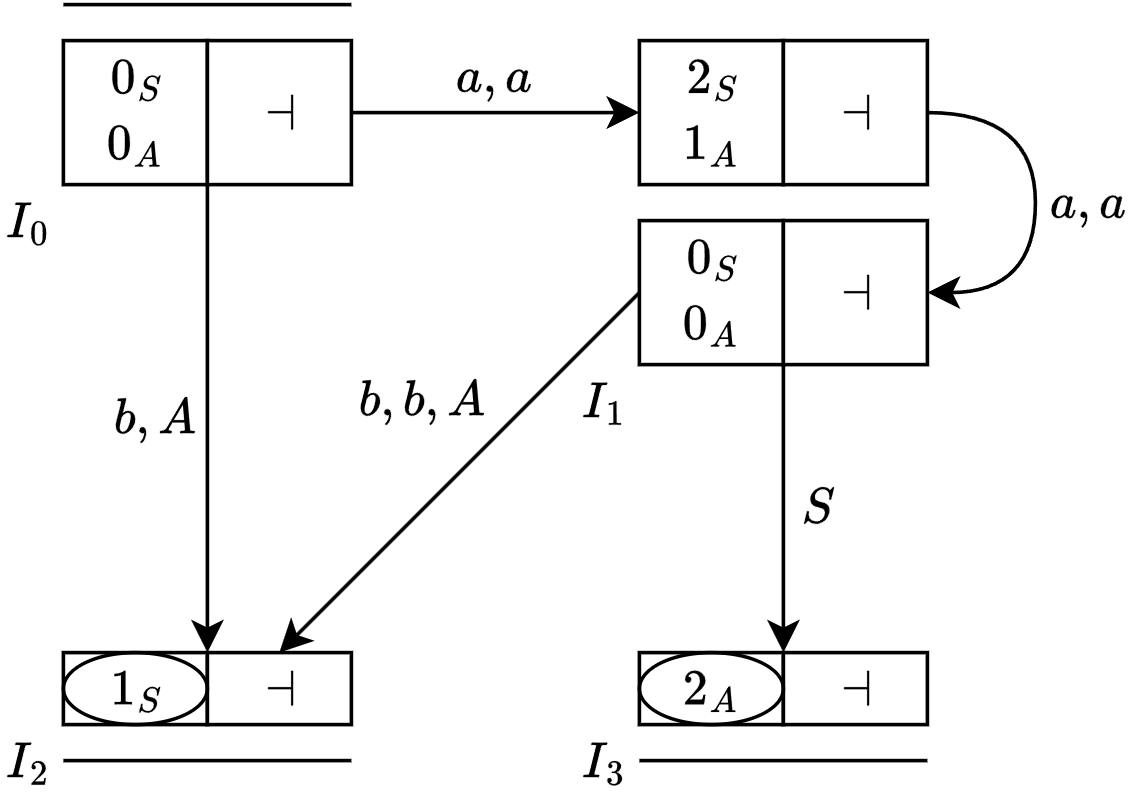
\includegraphics[width=0.5\linewidth]{images/synsol.png}
        \end{figure} 
        Notably, there are no reduce/reduce conflicts or shift/reduce conflicts.
        However, a convergence conflict arises from the $b$ transitions originating from the same $m$-state, converging in the same $m$-state, and sharing an identical symbol in both convergent states. 
        Consequently, the grammar is not ELR(1).
    \item The guide sets of the machine net, completed with call arcs to construct the Predictive Control Flow Graph (PCFG), are outlined below:
        \begin{figure}[H]
            \centering
            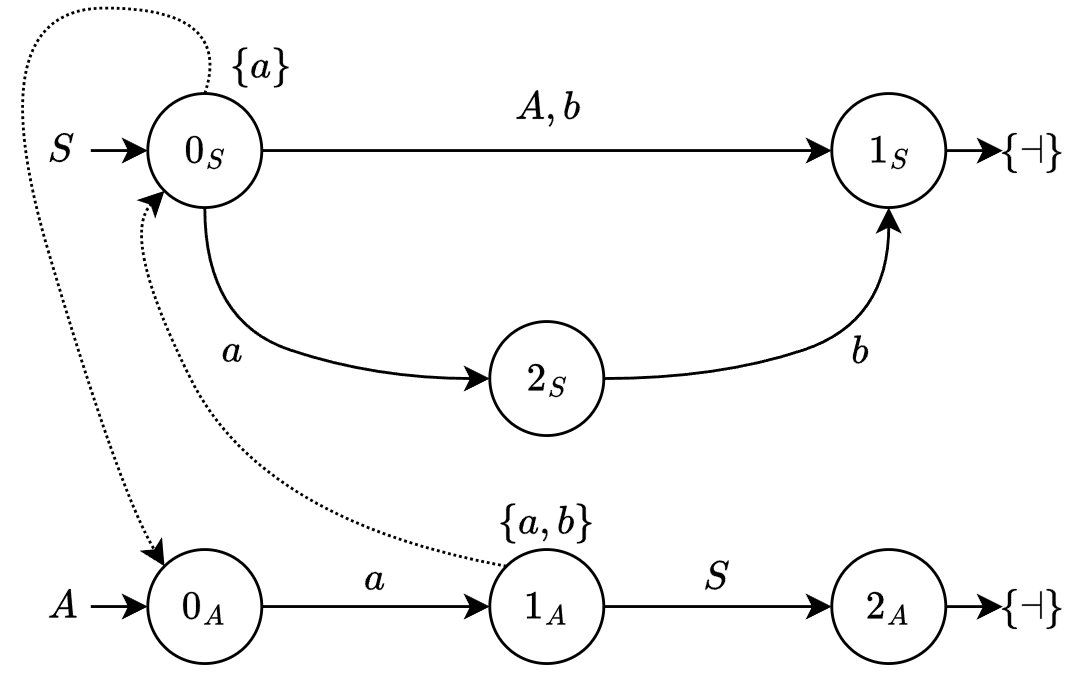
\includegraphics[width=0.45\linewidth]{images/PCFG.png}
        \end{figure} 
        The guide sets on the terminal shift arcs, although trivial, are not displayed. 
        The grammar is not ELL(1) due to overlapping guide sets at the bifurcation state $0_S$, indicating non-determinism.
    \item The Earley vector for the string $aab$ is presented below:
        \begin{figure}[H]
            \centering
            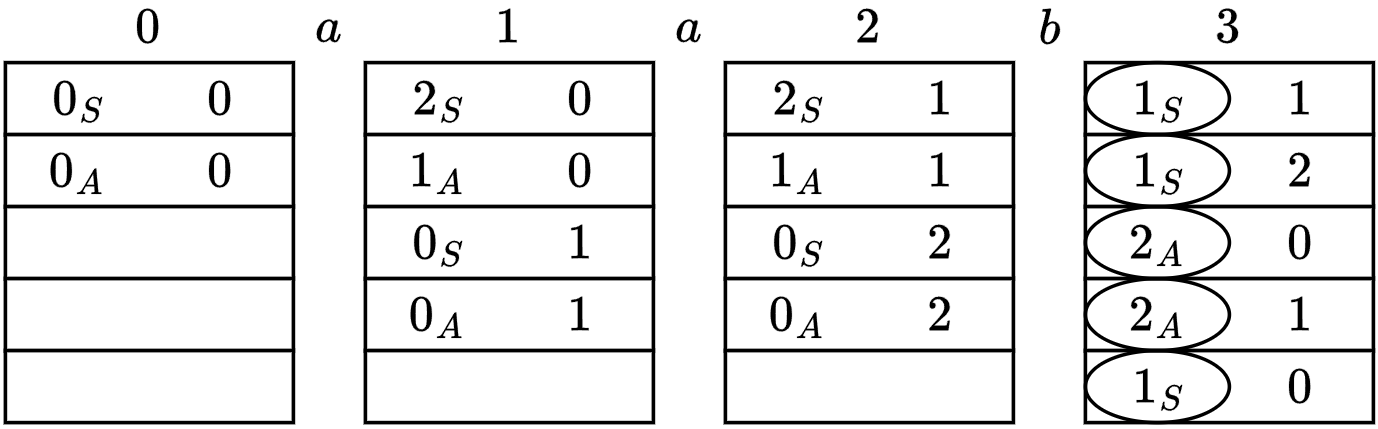
\includegraphics[width=0.65\linewidth]{images/earley.png}
        \end{figure} 
        The final item $\left\langle 1_S,0\right\rangle$ in the last vector element signifies the acceptance of the string $aab$ and corresponds to the two parsing trees associated with the string.
\end{enumerate}